\section{Tests}
\subsection{Zeitliche Analyse}
\subsubsection{Test Simulation mit System Viewer}
In Abb: \ref{fig4} wird eine Sequenz der Simulation während sich das Programm in einer Pause befindet, also keine Aufträge auszuführen sind, gezeigt. Diese Sequenz beginnt mit dem Beweger-Task (1.) welcher die virtuelle Position des Turms aktualisiert. Anschließend werden alle Sensor-Tasks nacheinander aktiv und überprüfen ob sich an ihrer Stelle gerade der Turm befindet und schreiben ihre Antwort darauf in die MessageQueue. Diese wird von dem Sensor-Collector, nachdem alle Sensoren durchgelaufen sind, ausgelesen und von diesem zu einem Gesamt-Konstrukt zusammengefügt und in die MessageQueue an die HRL-Steuerung geschrieben. \\
Das Gantt-Diagramm  Abb: \ref{gantt} wird damit bestätigt.

\begin{figure}[H]
	\centering
  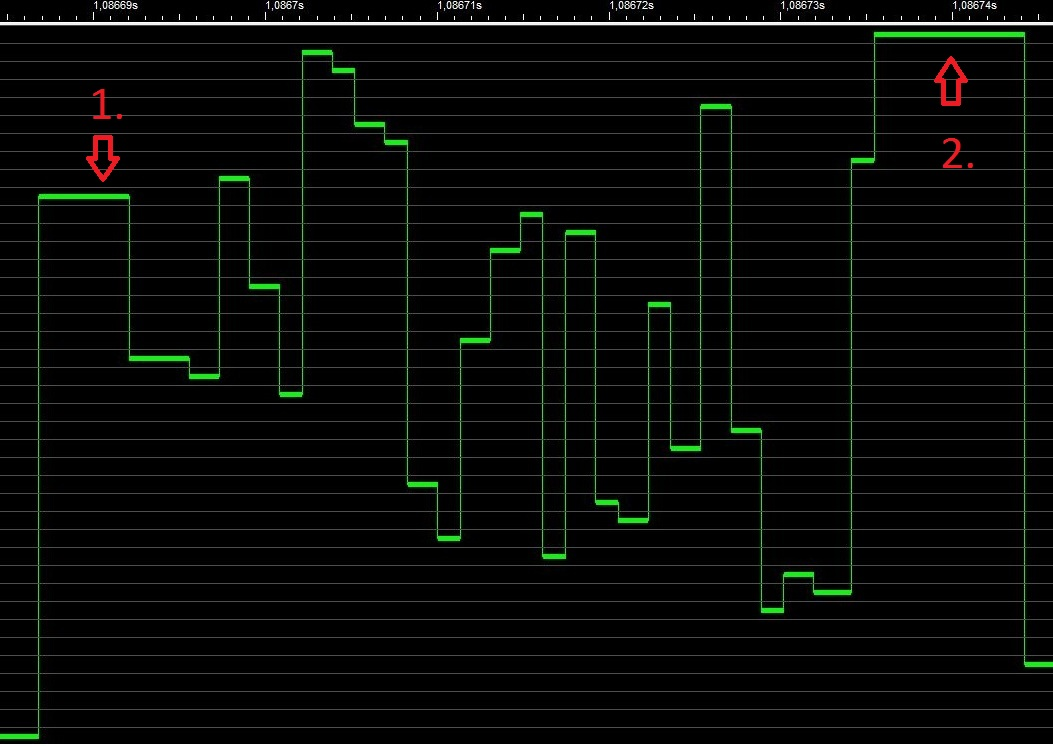
\includegraphics[width=\textwidth]{diagrams/simulation_erklaerung.jpg}
	\caption{Simulation mit System Viewer}
	\label{fig4}
\end{figure}
\subsubsection{Test Hochregal-Steuerung mit System Viewer}
Die Hochregal-Steuerung besteht aus lediglich zwei Tasks, welche sich wie in \todo{Gantt Diagramm} nicht unterbrechen. Der Movement-Task (1.) beginnt mit der Berechnung der Aktor-Befehle, welche anschließend von dem AktorPushData-Task(2.) an die Simulation weitergeleitet werden. Auch dieses ist somit Bestätigt.
\begin{figure}[H]
	\centering
  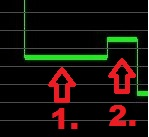
\includegraphics[width=0.5\textwidth]{diagrams/steuerung_zeit.jpg}
	\caption{HRL-Steuerung mit System Viewer}
	\label{fig5}
\end{figure}